\documentclass[]{article}
\usepackage{graphicx}
\usepackage{breakurl}
\usepackage{url}
\usepackage{algorithm,algpseudocode}
%opening
\title{Web scrapping techniques for price statistics -  the Romanian experience}
\pagenumbering{arabic}

\author{Bogdan Oancea$^1$ \and Marian Necula$^2$}
\date{%
	$^1$National Statistics Institute of Romania, bld. Libertatii no. 16, Bucharest, Romania, email: bogdan.oancea@insse.ro, phone: +40731302173, corresponding author\\%
	$^2$National Statistics Institute of Romania, bld. Libertatii no. 16, Bucharest, Romania, email: marian.necula@insse.ro\\[2ex]%
	\today
}

\renewcommand{\figurename}{Fig.}


\begin{document}


\maketitle

\begin{abstract}
Internet has been widely recognized as a new data source that can be used either to compile new statistics or to enhance the 
traditional ones in several fields of official statistics. Considering that online commerce has a rapid growing share in the 
overall household’s consumption expenditures behavior when selecting a distribution/transaction channel, price statistics is 
one of the research areas in official statistics which benefits greatly from this new data source. Since mid 2000, there have 
been several projects developed by official statistics national offices in order to explore the potential of collecting data 
through Internet and to enhance the current statistical production system, including the classical consumer price index (CPI). 
This paper provides a description of the Romanian National Institute of Statistics experience regarding the use of Internet 
as a data source and of an exercise in compiling an experimental CPI based on Internet data. The aim the pilot project was to 
investigate whether alternative data collection methods for price statistics can be introduced and enhance the statistical 
production system in the near future and, most important, it was a great firsthand opportunity to identify methodological 
challenges which are inherent. A chain of software tools was developed in order to automate, as much as possible the whole process. 
The tool chain is built on top of traditional methodology used for CPI, enhanced by new features such as simple clustering 
technique for treating high volatility present in the collected data using a distance-based method for classification similar products.
\end{abstract}

{\bf Keywords:} web scrapping, price statistics, data collection.

\section{Introduction}

For the past 30 years, the world has witnessed a new kind of fundamental structural change, which resembles, in terms of magnitude and impact, with the Industrial Revolution, as data production and usage was actively embedded in the very fabric of society. Data pervasiveness in every human and\\or non-human activity was made possible by the advent of new technologies such as the Internet and World Wide Web. This created an exponential increase in data generation, coined under the term Big Data. In 2013, at the DGINS conference in Scheveningen, Netherlands, the European Statistical System (ESS) Committee agreed upon the strategical importance of Big Data and set the stage for future plans on integrating Big Data into the official statistics production system \cite{mschv}. ESS Task Force Big Data was created and entrusted to setup a Big Data strategy and implementation framework. Along with other partners, the Big Data Action Plan and Roadmap 1.0. was elaborated as a planning and monitoring tool, providing descriptions of the necessary steps that should be undertaken by ESS and NSI's for an optimal response to this new challenge on short, medium and long-term. The ESSnet on Big Data, the collaborative research network of ESS, was tasked with piloting research projects \cite{awirth} to asses what are the necessary capabilities, such as new methodological approaches \cite{fricc}, new skills and new IT technologies, and also to design them. In 2017, The Romanian National Institute of Statistics started an internal project to asses the potential of data collection methods from the World Wide Web with some preliminary results being presented at the DGINS 2018, Bucharest Conference \cite{oancea}. Bucharest Memorandum \cite{mbch} explicitly expressed that new data sources, new IT technologies and new expertise will be at the core of Trusted Smart Statistics initiative \cite{ricwirskagiarei}, an Eurostat and ESS joint effort to incorporate Big Data sources into the statistical production system at ESS level.

The incorporation of Big Data sources in the official statistical production does not aim to entirely replace the traditional methodologies, but it is rather an iterative and incremental approach in which certain components of the traditional statistical production process are enhanced by the Big Data sources inputs and the related processing algorithms \cite{grif2016_1}, \cite{grif2016_2}. Alternatively, Big Data sources can contribute to the reduction of the response burden or they can be used only to study some economic or social phenomena before designing a statistical survey which are inherently expensive to pilot. Also, incorporating Big Data sources into official statistics means maintaining a net competitive advantage and relevance of the official statistics products compared to those provided by a plethora of commercial players, with reference to large corporations that are active in the field of information technology \cite{eu2012}.

One of the main big data sources is the World Wide Web (WWW) system, which can be considered an immense reservoir of information impossible to be neglected
by official statistics institutes. In order to take advantage of the data publicly available on Web sites some automatic procedure for data collection 
should be designed first. These procedures are referred to under the term of web-scrapping or automated data collection.

Automatic data collection of price data and its use to derive statistical indicators was pioneered by MIT \cite{MIT} where the prices collected 
from online shops were used to build a CPI for some South-American countries. Since this first experiment, several
statistical offices throughout the world started to collect data from online retailers and study how these data sets can be used
for CPI calculation. We can mention here Statistics Netherlands \cite{cbs}, ISTAT \cite{polidoro}  
or Destatis \cite{bruner} as some of the first statistical offices in Europe that experimented the web-scrapping technique for online prices, 
although they didn't follow the classical big data approach of MIT and only monitored some prices or tried to collect prices
only for the products included in the traditional collection method. The web-scrapping technique was used to collect data in other areas
of statistics too, for example to improve some statistical registers \cite{barcoli} or for job vacancies \cite{swier2}.
No matter how it was used, for bulk scrapping of all prices, or for only specific prices in certain areas \cite{cbs2} the web-scrapping technique 
proved to be a very useful method in the hand of statisticians.


Under these auspices, the overall objectives of our experimental project were to streamline the statistical production process by 
lowering the overall production costs, reduce the response burden and the dissemination term. Such projects, through the incorporation 
of modern computing technologies, could create the premises for developing a framework for testing and piloting new methodologies 
and technologies in a systematic and rigorous manner \cite{ons2017}. 


Our project experimented on how web-scrapping collection method can be used as an alternative tool for data collection in order to compute a new/experimental CPI or to improve upon the classical CPI computation \cite{otawa2017}. We started our work by identifying and 
selecting online channels that have significant weights in the process of trading goods and services for household consumption. 
This is not an easy task given that there is no information on the volume of online transactions made by firms, 
issue found in other projects too \cite{willenborg2017}. 
An example may be that retailers in the hypermarket category, although they have a physical trading correspondent with very high 
trading volumes, the volume of online transactions is unknown. The criteria used to select the online trading channels included in 
our study was to have a physical correspondent and record significant overall sales turnover at national level. Next, we proceeded with the 
task of identifying the appropriate means to implement the automated price collection process from e-commerce sites. The criteria 
used to identify the optimal solutions are expressed in terms of flexibility, ease of use, scalability and cost. An essential task 
to achieve this goal was to explore different methods/approaches and test the existing solutions. 


The second objective of our project was to carry out the automatic price collection process over a relevant period: 6 months - 2 years. 
Achieving a maturity level specific to official price statistics that are currently published will require a much wider period of 
rigorous and systematic testing of the collection process and the results obtained. The resources available for running the data 
collection, technology and skills are critical and a continuity plan should be devised if some data sources become unavailable, 
legislative changes occur during this period, or the technology and skills are outdated by the evolution of the Web architecture. 


The third objective of our project was to compute an elementary price index at article/varietal and assortment level and compare 
it with those obtained using the traditional data collection method in order to emphasize the issues related to the difficulties 
of applying and/or adapting the traditional CPI methodology \cite{cpi} to the new data sources.  A compromise to 
ensure a certain degree of comparability is the use of traditional CPI methodology \cite{cpi2}, \cite{cpi3} to estimate price indices, although 
traditional methodology may be incompatible from some points of view with the new data source. 


Last, but not least, we intended to identify the legally sensitive aspects regarding the reconciliation between National Statistical Law, the European Statistics Code of Practice, other regulations on official statistics and legislation on access to online data \cite{swier}.

The paper is structured as follows. In section \ref{section2} we present details of the data collection process, in section \ref{methodology} we provide a description of the methodological approach, in section \ref{results} we present our first results and section \ref{conclusions} concludes our paper.


\section{Data collection}\label{section2}
 
Some of the official statistics offices that run similar projects have opted to outsource this component to companies specialized 
in collecting, processing and storing the data instead of acquiring the data directly. While this minimizes greatly the overhead 
cost associated with developing and maintaining a large portion of the production pipeline. We explored several existing software solutions: 
Robot framework \cite{robot2018}, Scrapy \cite{scrapy1}, \cite{scrapy2} Apache Nutch \cite{nutch}, RSelenium \cite{rs1}, and \cite{rvest}. 

The observation unit was the web site of the retail companies. In this case, the assumption from which we started was 
that the companies cover the entire national territory through their site. Sites selection was based on establishing a 
sales-turnover relationship, sorting by decreasing order the sales figures reported by the firms that own the sites. 
At the present moment, there are certain barriers, for example the most important player in terms of turnover on the 
hypermarket segment in Romania, does not have a section dedicated to online transactions. We selected 4 sites for food, 
5 sites for clothing and 5 sites for footwear products. However, moves made at European level by firms that have physical 
stores on this segment suggest that market forces will require online migration of the most important players in the field.

Table \ref{table:1} provides a description of the collected variables. For each item we collected the item name, if provided, 
a quantitative and qualitative description of the item, current sale price, if provided, price unaffected by discounts or 
price per standardized quantity, name of the site from which the data was collected and date of collection. Data is stored 
in comma separated values files. In total, between 50,000 to 70,000 records were collected each month.

\begin{table}[h!]
	\centering
	\begin{tabular}{ c c c p{0.4\linewidth}}
		\hline
		 No. Crt. & Variable Name & Type & Definition  \\
		\hline  
		1 & \texttt{prod\_name} & string & Records the name of the item as seen on site.\\  \hline
		2 & \texttt{prod\_des}  & string & Auxiliary information regarding item quantitative and qualitative specifications. \\ \hline
		3 & \texttt{price}	  	& float  & Price of the item as seen on site.  \\ \hline
		4 & \texttt{price\_old} & float  & Price unaffected by promotions or price per quantity.\\ \hline
		5 & \texttt{site}	  	& string & Name of the site. \\ \hline
		6 & \texttt{date} 	  	& date   & Collection date. \\ 
		\hline
	\end{tabular}
	\caption{Collected variables description}
	\label{table:1}
\end{table}

Data collection took place through the Robot Framework and RSelenium software solution. 
After we evaluated several web scrapping frameworks we started our project using Robot Framework. This software solution is implemented using Javascript language with node.js library.
The main advantage of this framework is that it can automatically access asynchronous and dynamic web content by simulating the interaction between a user / web browser and a web server. Automating the collection of information from dynamically generated content sites involves simulating the interaction between the user/web browser and the server through a headless browser application, in this case phantom.js. The Robot Framework solution allows user to set up a script that sends asynchronous requests to the Web server through the browser. Content of responses sent asynchronously by the server are stored, parsed, and copied to .csv files. Depending on the nature and amount of the dynamic elements in a website, a web scraping session may take between a few minutes and a few hours.
Editing the script file involves the use of information available through a web developer tool, common to all major Web browser distributions (Chrome, Firefox, Edge), for identifying the item of interest from the Web page structure, as well as any scripts that can interact with that item. The address of an item in a document can be reproduced in two ways within the script file, the first being with the CSS selectors and the other with the Xpath selectors. The difference between the two modes is given by the fact that the second one can point to text content components within the element. Extracted page URLs are provided to a set of procedures that serialize navigation process on Web sites. It is worth mentioning that the Robot Framework solution is highly configurable, through the introduction of Javascript specific procedures that are used by the sites, proven to be a scalable web scrapping solution for the requirements of a medium sized project. The major downside of Robot Framework is that currently, from what we are aware is not under active developement.

RSelenium \cite{rs1} is an API developed as a R package for the popular Selenium automation web browser testing framework \cite{}. RSelenium provides basic methods for passing synchronous/asynchronous messages and parsing responses to and from a web browser. A net advantage of using RSelenium consists in how easy is to integrate into the R ecosystem, substantially improving the maintainability aspects of the whole process. For example, creating scripts that can access web sites/web pages in parallel \cite{dopar}\cite{foreach} is very easy to implement and maintain, by comparison with other web scraping solutions, saving countless hours in the data collection process. A basic work pipeline consists in allocating computational power for a parallel cluster, starting a Selenium server instance, starting multiple web browser instances, navigating and collecting data, closing the web browsers, the server and the nodes after each successful session or saving the browser state as a message in case of exception.   

\begin{algorithm}[h]
	\caption{Algorithm for data collection}
	\label{alg:dc}
	\begin{algorithmic}
		\State Read $URL's$
		\State Detect cores
		\State Allocate Cluster
		\For{each $URL$}
		 \State Start $node$
		 \Procedure{Recursion}{$URL$}
		 		\If{$URL$ is dead}
		 			\State\Return
		 		\Else
		 			\State Visit URL
		 			\State $text \gets get\_html[URL]$
		 			\State $URL  \gets get\_url[text]$
		 			\State $Data \gets get\_content[text]$
		 			\State \Return \textsc{Recursion}{($URL$)}
		 		\EndIf
			\State Write $Data$
			\EndProcedure
		  \State Stop $node$
		\EndFor	
	\end{algorithmic}
\end{algorithm}





The automatic collection of prices observed on the sites included in the sample was made during
the same period as for the traditional CPI survey. Due to the noise present in extracted data, decomposition at the core components of the CPI classification is required first.


The structure of the data collected from the retailers’ sites for the food group of products contains the product 
name, the manufacturer, the quantity, certain technical-quality details, the price per unit or the price per piece, 
the article/varietal and assortment type, and the category according to the structure of the site. From the point of view 
of the classification of products in a given product category, these data may appear at a first glance 
as inputs for a manual or automatic classification procedure, but the very large number of products and the fact 
that the description is not standardized for all sites targeted by the collection process makes this stage to be considered as the most difficult one.

A trivial observation about the form of data is that they cannot be directly used in the process of classifying 
and estimating price indices. To address this issue, we have developed a series of R scripts that transform 
the data in a way that allows flexible handling. The CPI computation steps are sequentially deployed, the data 
input for each stage depending on the output of the previous stage, except for the first step whose input depends 
on the result of the automatic data collection.



In the following, the activities carried out at each stage will be detailed, noting that we attempted to keep the 
traditional CPI methodology as much as possible intact. A graphical representation of the data collection and processing is shown in \ref{fig:6}.

\begin{figure}
\centering
\includegraphics[height=0.7\linewidth]{fig6.eps}
\caption{Data collection and processing session}
\label{fig:6}
\end{figure}


The first activity was the data cleaning. We started with 
the web scrapped files and performed some basic operations checking for missing data and other basic validation operations. 
In case there are missing items among the data sets, the web-scrapping process resumes, after checking the online accessibility 
of the site and the log files of the web-scrapping application. Some possible error sources could be: 
\begin{itemize}
\item sites were unavailable or have undergone changes;
\item the web-scrapping application encountered web content elements that cannot be directly processed;
\item web server identified the web-scrapping application as a malicious software and imposed an access restriction to the site at the IP address level.
\end{itemize}


Next, all the files obtained from the data collection process for a certain month are joined automatically. The resulting 
file is read by an R script and transformed into a data structure suitable for an automatic processing procedure. Some 
basic transformations are again performed using an automated R script, before classifying and linking the products according 
to the CPI classification. We started with the manual product linking and classification according to the standard CPI 
classification which implies identifying the observations which contain a description similar to the one provided in the
classical CPI classification. This activity can generate errors whose propagation can significantly influence the quality 
of the results. The principle that we used in the absence of a previous experience in working with methodological aspects 
for product selection was to assume that the consumer will choose a product or products substitutable to the one present 
in the standard classification within a reasonable price limit ($<= 150\%$ of the price of an article from the standard classification). 

Thus, we chose to select several articles for one assortment within the same observation point. To reinforce the strict tracking 
rule of the same articles found in the standard CPI methodology, we performed join operations between the data structures 
for all decades and observed months. The join operation between two or more tables was based on the "name" variable containing 
the product description by matching strings in a 1 to 1 ratio. After performing this activity, from an initial number 
of about 10,000 of articles, they were restricted to 545 articles, 216 assortments, and 52 expenditure groups, 
identified as constant during the 6 months of observation, assuming that the description given in the observations 
made for the variable "name" represents a guarantor for the invariance of the technical and qualitative characteristics of the targeted products.


Several attempts were made to develop an automatic classification procedure with encouraging results. However, their use 
would involve deviations from the classical CPI methodological framework, manifested by the appearance and disappearance 
of the articles in the sample with a high frequency. We tried several machine learning and distance-based algorithms 
for this procedure and the results are presented in table 1. The best results, as it can be observed in \ref{table:2}, 
were obtained using the Levenshtein distance.


\begin{table}[h!]
\centering
\begin{tabular}{ c c }
	\hline
	Algorithm & Accuracy \\
	\hline  
	Boosting & 0.56 \\  
	Support Vector Machines & 0.34 \\
	Random Forests &  0.41 \\
	Scaled linear discriminant analysis & 0.17 \\
	Bagging & 0.28 \\
	Regex & 0.70 \\
	Levenstein Distance & 0.80 \\
	\hline
\end{tabular}
\caption{A summary of the methods used for automatic classification}
\label{table:2}
\end{table}

\section{Some methodological aspects}\label{methodology}

A secondary objective of the project is to asses if online observed prices can be successfully
used as a substitute data set for computing, either the traditional CPI or a similar 
experimental statistics, e.g. online observed CPI. Therefore, in order to retain, 
as much as possible, comparable results with the traditional CPI, the collection periods 
within a month, along with the goods and services included in the CPI national classification 
were preserved. Due to practical limitations regarding the allocated resources for 
this project, the data collection process was focused on food and beverages and items 
covering clothing and footwear categories, as these types of goods hold the biggest share in 
household's consumption expenses, e.g. food accounts for nearly 40\% of total expenses\cite{hhs}. 

CPI is computed by weighted serial aggregation of elementary price indices at item, assortment, 
category and group level, the entire process being a combination of traditional procedures\cite{cpi} 
and intermediate aggregations targeted at product survivability from one period to another. 
The process is being graphically described by \ref{fig:2}. After data pre-processing, i.e. testing 
if data is consistent with the computation requirements, removing duplicates, matching 
products across different periods, the first step requires prices aggregation into an arithmetic 
monthly average for each item, given that data was collected 3 times per month for food and 
beverages and once per month for clothes and shoes. 

\begin{equation}\label{eq:1}
\overline{p}_{v} = \frac{\sum_{j=1}^n {p_{v_{j}}}}{n} ,
\end{equation} ,

\begin{center} 	
	\overline{p}_{v} &= monthly price average for any given variety, \\
	n &= number of periods for which the price data was collected in a given month, \\
	p_{v_{j}} &= price of an item in $j^{th}$ period within a month	
\end{center}

The average is used to compute elementary 
price indices at product/variety level, by dividing the current monthly average for an item to it's respective base period monthly average. 

\begin{equation}\label{eq:2}
i_{p_{v}} = \frac{\overline{p}_{v_{current}}}{\overline{p}_{v_{base}}} ,
\end{equation}

\begin{center}	
	$i_{p_{v}}$ = elementary prices index for any given variety, \\
	$\overline{p}_{v_{current}}$ = current monthly price average, \\
	$\overline{p}_{v_{base}}$ = base monthly price average.
\end{center} 

To ensure that results are comparable at different periods and capture only pure price change, ideally would be to collect price data for the same products indefinitely\cite{cpi2}. In the real world, this is impractical due to different reasons. Therefore, price data collectors are equipped with a list of strict rules when products or services are no longer available and substitutes are needed. These rules may target product description(producer, weight, composition, etc.), store placement and local/national market share, or a combination of these is used to ensure that qualitative differences between products no longer available on the market and substitutes are minimal \cite{cpi}. According to different research studies on using Big Data to compile CPI conducted inside National Statistical Offices, item survivability in sample is the most common issue in preserving comparable results across longer periods\cite{ons2017, willenborg2017, tranzitivity, kints}. To address this issues an intermediate calculation step was necessary. Based on the optimal supervised classification score, price indices for similar items were clustered into a generic price index for the same statistical unit by using a geometric mean. For example, within the same statistical unit we collected at $t_{0}$ 3 products, according to the classification score, and at $t_{1}$ 2 products for the same assortment, to ensure the price change is kept within reasonable margins, we apply a geometric mean to cluster them into a generic product.   

\begin{equation}\label{eq:3}
i_{g} = \sqrt[n]{\prod_{j=1}^{n} i_{p_{v_{j}}}}
\end{equation}

\begin{center}
	$i_{g}$ = elementary price index for a generic product, \\
	$n$ = number of products within the same assortment based on the classification score, \\
	$i_{p_{v_{j}}}$ = the $j^{th}$ elementary price index within the same assortment
\end{center}

The subsequent calculations follow roughly the steps as in the Romanian National Institute of Statistics CPI methodology\cite{cpi}. taking into consideration that in order to obtain the price index at the expenditure category level, e.g. items containing white flour, we assigned to each category a weight equal to $\frac{1}{n}$,
where $n$ is the number of assortments identified as belonging to the same category. 

\begin{equation}\label{eq:4}
i_{a} = \sqrt[n]{\prod_{j=1}^n i_{g_{j}}}
\end{equation}

\begin{center}
	$i_{a}$ = price index for an assortment, \\
	$n$ = number of statistical units per assortment, \\
	$i_{g_{j}}$ = elementary price index for a generic item in the $j^{th}$ statistical unit
\end{center}


\begin{equation}\label{eq:5}
i_{c} = \frac{\sum_{j=1}^n i_{a_{j}}}{n}
\end{equation}

\begin{center}
	$i_{c}$ = price index for a category
	$n$ = number of assortments in the category, \\
	$i_{a_{j}}$ = the $j^{th}$ price index within an assortment
\end{center}

To obtain indices at group level, e.g. foods, in the last step, we used COICOP consumption weights from CPI methodology in order to aggregate category indices.  The following formula was used:


\begin{equation}\label{eq:6}
cr_{w_{g}} = \frac{\sum_{j=1}^{n_{c}}{w_{j_{c}}}}{\sum_{j=1}^{n_{b}}{w_{j_{b}}}}
\end{equation}

\begin{center}
	$cr_{w_{g}}$ = re-calibration coefficient for group weights, \\
	$n_{c}$ = current period number of categories belonging within a group, \\
	$n_{b}$ = base period number of categories belonging within a group, \\
	$w_{j_{c}}$ = the $j^{th}$ group weight for current period, \\
	$w_{j_{b}}$ = the $j^{th}$ group weight for base period
	
\end{center}

The re-calibration coefficient is applied to each category weight:

\begin{equation}\label{eq:7}
  w_{r} = w_{g} \times cr_{g}
\end{equation}

\begin{center}
	$w_{r}$ = re-calibrated weight, \\
	$w_{g}$ = initial weight, \\
	$cr_{g}$ = re-calibration coefficient
\end{center}

This intermediate stage is necessary due to potential absence of certain items from sample at any given moment in time, 
The final formula used was:

\begin{equation}\label{eq:8}
	i_{g} = \sum_{j=1}^{n} i_{c_{j}} \times w_{r_{j}}
\end{equation}

\begin{center}
	$i_{g}$ = price index at group level, \\
	$n$ = number of categories within a group, \\
	$i_{c_{j}}$ = price index of the $j^{th}$ category, \\
	$w_{r_{j}}$ = re-calibrated weight for the $j^{th}$ category
\end{center}

The process diagram is shown in Fig. \ref{fig:1}, while in Fig. \ref{fig:2} we build a process diagram in terms of GSBPM (Generic Statistical Business Process Model)\cite{gsbpm}. The GSPBM framework was used to attain a small, but relatively modular production pipeline, as a monitoring and integration tool and, also, as a checklist in producing some preliminary results. Starting with some basic objectives, we tried to identify critical points in the production pipeline and provide flexible definitions for a set of activities flagged as important. While not present in the diagram, the entire workflow chain contains feedback loops between each state and on the state itself, in order to build incremental improvements taking into consideration the allocated resources. Depending on future needs, the entire pipeline can be subjected to re-engineering.      


\begin{figure}
\centering
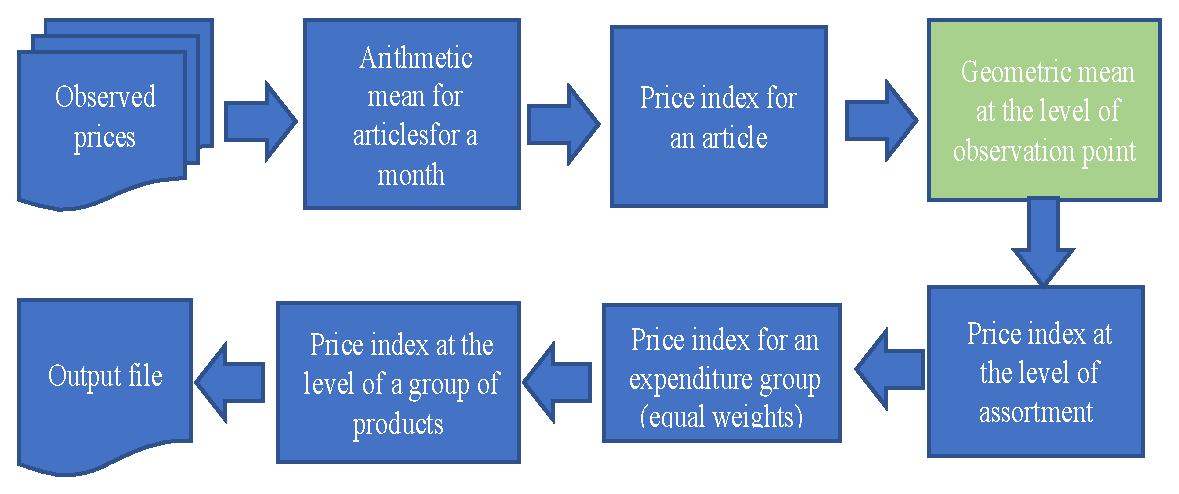
\includegraphics[width=0.8\linewidth]{fig1.eps}
\caption{The process diagram for computing online price index - the green box adds a new phase to the traditional price index methodology}
\label{fig:1}
\end{figure}


\begin{figure}
\centering
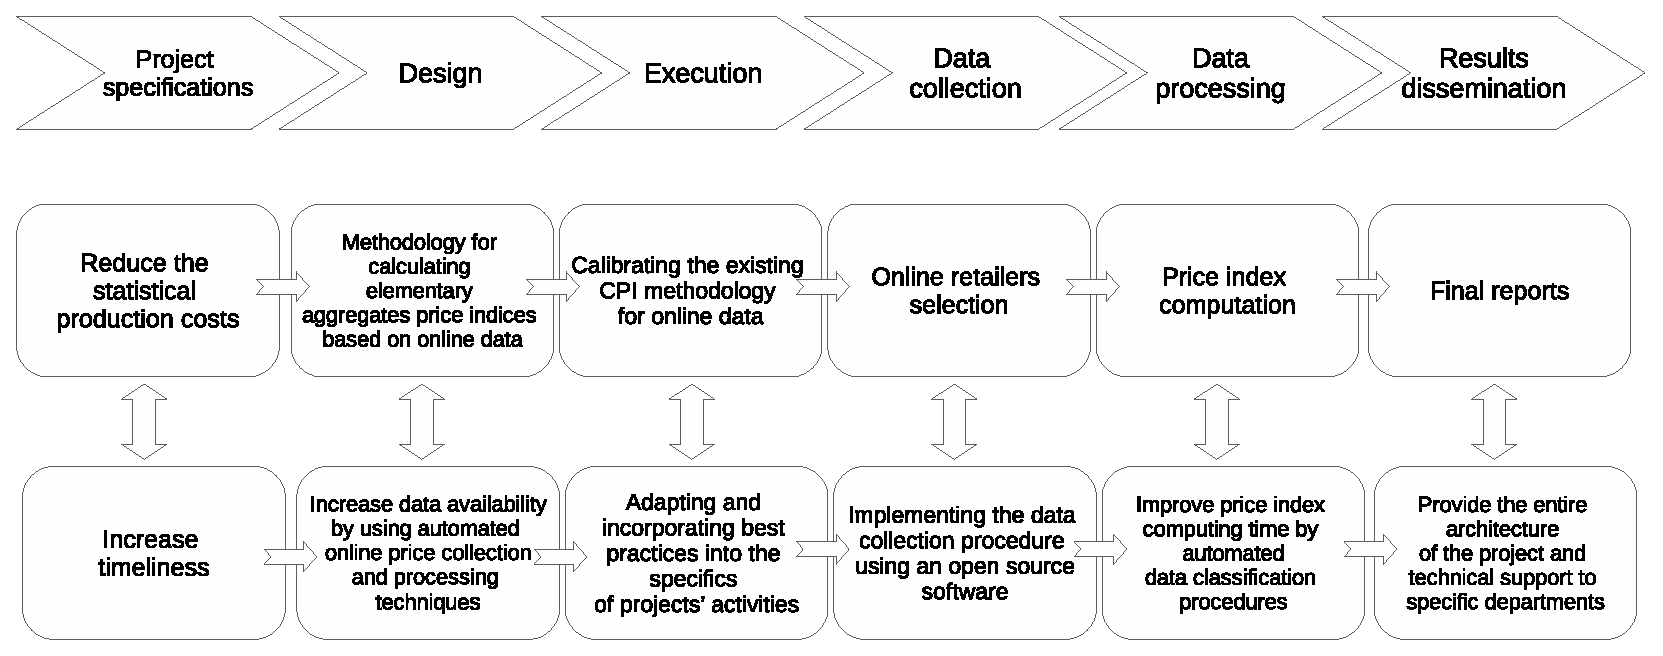
\includegraphics[width=1\linewidth]{fig2.eps}
\caption{The GSBPM diagram}
\label{fig:2}
\end{figure}



\section{Results and discussion } \label{results}


Using August 2017 as the basis for computation of the monthly price index, we obtained the aggregated indices at the 
groups of food, clothing and footwear presented in figures \ref{fig:3}, \ref{fig:4}, and \ref{fig:5}.


\begin{figure}
\centering
\includegraphics[width=0.7\linewidth]{fig3.eps}
\caption{The comparative evolution of the price indices for food}
\label{fig:3}
\end{figure}


\begin{figure}
\centering
\includegraphics[width=0.7\linewidth]{fig4.eps}
\caption{The comparative evolution of the price indices for clothes}
\label{fig:4}
\end{figure}


\begin{figure}
\centering
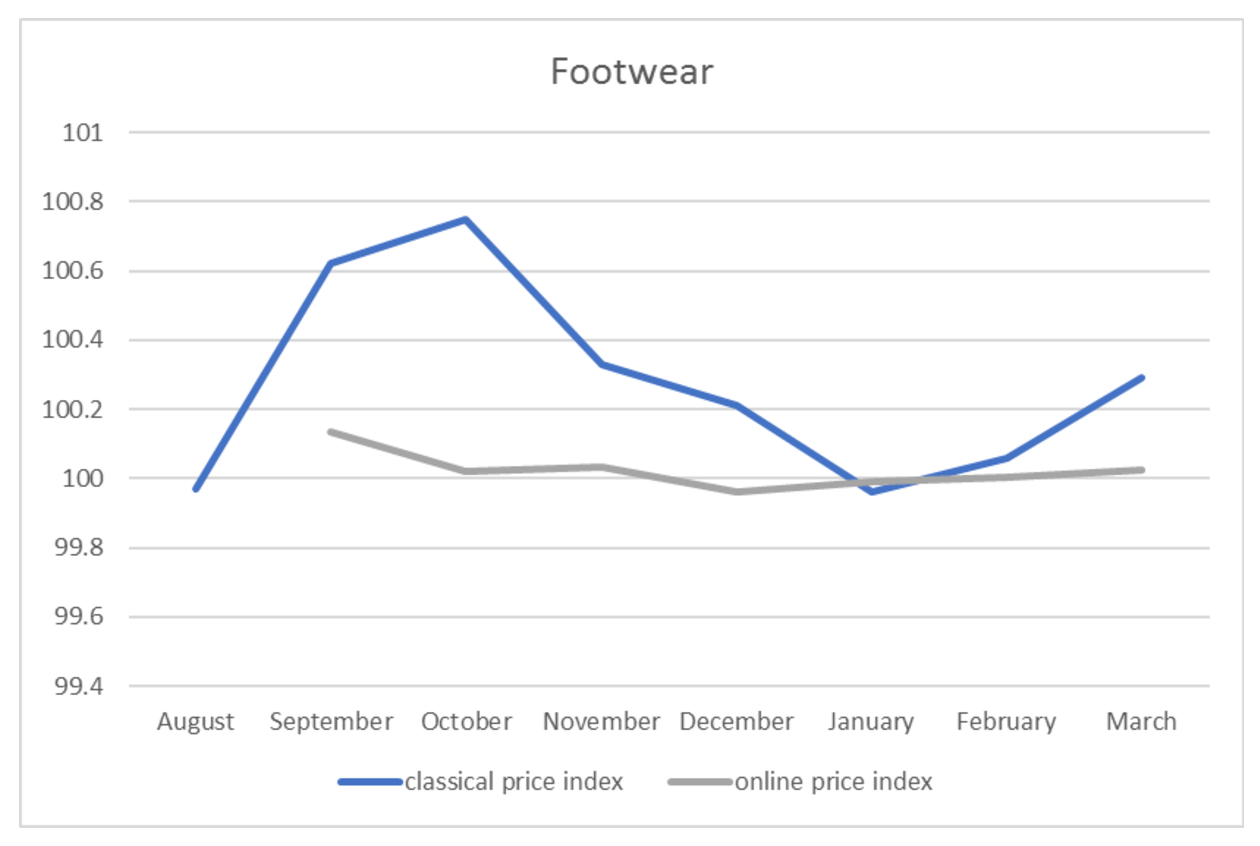
\includegraphics[width=0.7\linewidth]{fig5.eps}
\caption{The comparative evolution of the price indices for footwear}
\label{fig:5}
\end{figure}


From the evolution of the two price indices considered, it can be noticed that the online 
collection method implies a different trajectory due to the different samples used and the use 
of equal weights at assortment and expenditure group level. Another possible explanation can be found 
in the non-probabilistic sampling process through which online stores are selected ignoring the 
representativeness at national level due to the lack of specific information. Selected food, 
clothing and footwear stores can serve large cities and neighboring areas, having complex pricing 
policies which are different from small shops serving small city areas and rural communities.


\section{Conclusions and future developments}\label{conclusions}

This project was the first experiment that implemented a web-scrapping technique for data collection 
inside Romanian National Institute of Statistics. CBS's Robot Framework proved to be a very flexible web scraping tool, providing an easy solution
for developing and maintaing code just for data collection. The major drawback is that currently is no longer
in public active developement. RSelenium, along with other packages from R ecosystem, is a very powerful but easy to 
use tool, greatly enhancing the flexibility through the use of a single programming language for the whole workflow pipeline.  
While we gained experience with the software tools, we also 
identified some limitations for our specific study of online price collection which are briefly described below:
\begin{itemize}
\item Generalization hypothesis of online transactions. The number of households purchasing an 
online product is relatively small, and generally depends on several factors such as the geographical position, 
income level, education level, etc.
\item Not all businesses with a significant volume of transactions included in the list of observation 
units for traditional CPI has a website;
\item The IT technology can have a significant impact on price variation. An example of this may be the discrimination 
based on the geographic position of a user when displaying prices on a particular site;
\item The components of the classical consumer basket and the weights used at the level of the expenditure groups do not 
entirely reflect the consumption patterns and the budget restrictions of the population segment addressed by online stores.
\end{itemize}


Based on the results obtained and the potential of the web-scrapping collection method we intend to try and implement 
in other official statistics areas and we will continue to develop a specific/experimental online consumer price index [13], 
by extending the current collection procedures to the entire products and services nomenclature and by 
developing a new methodology based on the characteristics of the collected data. Secondly, a separate product and service nomenclature may 
be developed specifically for online data based on measurements such as the longevity of certain products 
and services in the online offer, and a series of metadata related to those products and services, for example, analysis of 
online interaction based on buyers reviews with the respective brands and the online store.


\begin{thebibliography}{99}
\bibitem{grif2016_1}
~Griffioen R, ten ~Bosch O, ~Hoogteijling E. Challenges and solutions to the use of internet data in the Dutch CPI. 
Workshop on Statistical Data Collection, The Hague, The Netherlands; 2016 [Cited 2019 Jun 27]. Available from: \url{https://www.unece.org/fileadmin/DAM/stats/documents/ece/ces/ge.44/2016/mtg1/WP2-3_Netherlands_-_Griffioen_ap.pdf}.

\bibitem{grif2016_2}
Griffioen R, ten Bosch O. On the use of Internet data for the Dutch CPI,
Conference of European Statisticians, Geneva, 2-4 May; 2016 [Cited 2019 Jun 24]. Availbale from : \url{http://www.unece.org/fileadmin/DAM/stats/documents/ece/ces/ge.22/2016/Session_2_Netherlands_on_the_use_of_internet_data_for_the_Dutch_CPI.pdf}.

\bibitem{eu2012}
European Commission. Internet as a data source. Luxembourg: Publications Office of the European Union; 2012.

\bibitem{ons2017}
Bhardwaj H, Flower T, Lee P, Mayhew M. Research indices using web scraped price data: August 2017 update, ONS, UK; 2017 [Cited 2019 Jul 1st]. Available from:
\url{https://www.ons.gov.uk/economy/inflationandpriceindices/articles/researchindicesusingwebscrapedpricedata/august2017update}.

\bibitem{otawa2017}
Auer J, Boettcher I, From price collection to price data analytics. How new large data sources require price statisticians to re-think their index compilation procedures. Experiences from web-scraped and scanner data.
Ottawa Group - International Working Group on Price Indices; 2017 [Cited 2019 May 15]. Available from: \url{http://www.ottawagroup.org/}.

\bibitem{willenborg2017}
Willenborg L. Elementary price indices for internet data. Discussion Paper no. 8, CBS, The Hague, Nederlands; 2017 [Cited 2019 Jun 15]. Available from:
\url{https://www.cbs.nl/-/media/_pdf/2017/25/elementary price indices.pdf}.

\bibitem{robot2018}
CBS. Robot Framework. 2018 [Cited 2019 Jan 20]. Available from: \url{http://research.cbs.nl/Projects/RobotFramework/index.html}.

\bibitem{scrapy1}
Kouzis-Loukas D. Learning Scrapy - Second Edition, Packt Publishing; 2018.

\bibitem{scrapy2}
Myers D, McGuffee JW. Choosing Scrapy. Journal of Computing Sciences in Colleges 2015; 31(1):83-89.

\bibitem{nutch}
The Apache Software Foundation. Nutch, a highly extensible, highly scalable Web crawler; 2018 [Cited 2019 Jun 12]. Available from:
\url{http://nutch.apache.org/}.

\bibitem{rvest}
Wickham H. rvest: Easily Harvest (Scrape) Web Pages {R package version 0.3.2}; 2016 [Cited 2019 Apr 2nd]. Available from:
\url{https://CRAN.R-project.org/package=rvest}.

\bibitem{cpi}
INS Romania. Ancheta statistică a preţurilor de consum al populaţiei (in Romanian); Bucharest: National Institute of Statistics; 2017.

\bibitem{cpi2}
ILO/IMF/OECD/UNECE/Eurostat/The World Bank. Consumer price index manual: Theory and practice. Geneva: International Labour Office; 2004.

\bibitem{cpi3}
UNECE/ILO/IMF/OECD/EUROSTAT/The World Bank/ONS. Practical Guide to Producing Consumer Price Indices. New York and Geneva: United Nations; 2OO9.


\bibitem{swier}
Swier N. How should web scraping be organised for official statistics? 61st ISI World Statistics Congress, Marrakech; 2017.


\bibitem{tranzitivity}
Willenborg L. Transitivizing elementary price indices for internet data using the cycle method. Discussion Paper, CBS, The Hague, Nederlands; 2017 [Cited 2019 Jun 1]. 
Available from: \url{https://www.cbs.nl/-/media/_pdf/2017/25/transitivizing elementary price indices.pdf}.


\bibitem{rs1}
Harrison J. RSelenium: R Bindings for 'Selenium WebDriver'. R package version 1.7.5; [Cited 2019 Jun 1] 2019. Available from :
\url{https://CRAN.R-project.org/package=RSelenium}.


\bibitem{MIT}
Cavallo A. Scraped Data and Sticky Prices. MIT Sloan Research Paper No. 4976-12; 2010.


\bibitem{cbs}
Hoekstra R, ten Bosch O, Harteveld F. Automated data collection from web sources for official statistics: First experiences. 
Statistical Journal of the IAOS. 2012; 28(3-4):99-111.

\bibitem{cbs2}
ten Bosch O, Windmeijer D, van Delden A, van den Heuvel G. Web scrapping meets survey design: combining forces,
BigSurv Conference, October 25 - 27, Barcelona, Spain; 2018.


\bibitem{polidoro}
Polidoro F, Giannini R, Lo Conte R, Mosca S, Rossetti F. Web scraping techniques to collect data on consumer electronics and airfares for Italian HICP compilation. Statistical Journal of the IAOS. 2015;31(2):165–176.
2015.

\bibitem{bruner}
Brunner K. Automated price collection via the internet. DESTATIS; 2014.

\bibitem{barcoli}
Barcaroli G, Scannapieco M, Scarno M, Summa D. Using Internet as a Data Source for Official Statistics: a Comparative Analysis of Web Scraping Technologies.
New Techniques and Technologies for Statistics, Bruxelles; 2015.


\bibitem{swier2}
Swier N. Webscraping for Job Vacancy Statistics. Eurostat Conference on Social Statistics:Towards more agile social statistics. Luxembourg; 2016.

\bibitem{hhs}
INS Romania. Coordonate ale nivelului de trai in Romania (in Romanian); 2019. [Cited 2019 Jun 1] Available from:
\url{http://www.insse.ro/cms/sites/default/files/field/publicatii/coordonate_ale_nivelului_de_trai_in_romania_2018_1.pdf}

\bibitem{kints}
van Kints M, de Haan J, Webster M. Utilising big data and multilateral index methods to produce the Australian CPI: Theory, implementation and empirical results. Statistical Journal of the IAOS. 2019; pre-press

\bibitem{gsbpm}
UNECE, Generic Statistics Business Process Model; 2014. [Cited 2019 Jun 1] Available from:
\url{https://statswiki.unece.org/display/GSBPM/GSBPM+v5.0}

\bibitem{dopar}
Calaway R, Microsoft Corp., Weston S, Tenenbaum D. doParallel: Foreach Parallel Adaptor for the 'parallel' Package {R package version 1.0.14} ; 2018. [Cited 2019 Jun 1] Available from: \url{https://cran.r-project.org/web/packages/doParallel/index.html}

\bibitem{foreach}
Calaway R, Microsoft Corp., Weston S. foreach: Provides Foreach Looping Construct for R {R package version 1.4.4}; 2017. [Cited 2019 Jun 1]
Available from: \url{https://cran.r-project.org/web/packages/foreach/index.html}  

\bibitem{mschv}
European Statistical System Committee, Scheveningen Memorandum Big Data and Official Statistics, 2013. [Cited 2019 Jun 1]
Available from: \url{https://ec.europa.eu/eurostat/documents/42577/43315/Scheveningen-memorandum-27-09-13}

\bibitem{mbch}
European Statistical System Committee,  Bucharest Memorandum on Official Statistics in a Datafied Society (Trusted Smart Statistics), 2018. [Cited 2019 Jun 1]
Available from: \url{http://www.dgins2018.ro/wp-content/uploads/2018/10/The-Bucharest-Memorandum-on-Trusted-Smart-Statistics-FINAL-1.pdf}

\bibitem{bdar}
Eurostat Task Force on Big Data, Big Data Action Plan and Roadmap 1.0, 2014. [Cited 2019 Jun 1]
Available from:
\url{https://ec.europa.eu/eurostat/cros/system/files/ESSC%20doc%2022_8_2014_EN_Final%20with%20ESSC%20opinion.pdf} 

\bibitem{awirth_1}
Wirthmann, A Big Data im Europäischen Statistischen System, AStA Wirtschafts- und Sozialstatistisches Archiv, 10, 2016; [Cited Jun 1]
Available from:
\url{https://link.springer.com/article/10.1007/s11943-016-0195-z}

\bibitem{awirth_2}
Wirthmann, A Trusted Smart Statistics: A reflection on the future of (Official) Statistics, European Conference on Quality in Official Statistics, Krakow, Poland 2018; [Cited Jun 1]
Available from:
\url{https://www.q2018.pl/session-27/}

\bibitem{fricc}
Ricciato, F Towards a Reference Methodological Framework forprocessing MNO data for Official Statistics, 15th Global Forum on Tourism Statistics, Cusco, Peru, 2018; [Cited Jun 1]
Available from:
\url{http://www.15th-tourism-stats-forum.com/pdf/Papers/S3/3_1_A_Reference_Methodological_Framework_for_processing_mobile_network_operatordata_for_official_statistics.pdf}

\bibitem{oancea}
Oancea, B Using Web scrapping techniques for price statistics -the Romanian experience, DGINS Conference, Bucharest, Romania, 2018; [Cited Jun 1]
Available from:
\url{http://www.dgins2018.ro/wp-content/uploads/2018/10/05-RO-Using-Web-scrapping-techniques-for-price-statistics.pdf} 

\bibitem{ricwirskagiarei}
Ricciato, F Skaliotis, M Wirthmann, A Giannakouris, K Reis, F Towards a Reference Architecture for Trusted Smart Statistics, DGINS Conference, Bucharest, Romania, 2018; [Cited Jun 1]
Available from:
\url{http://www.dgins2018.ro/wp-content/uploads/2018/10/07-ES-RO-mobile_network_datav3.pdf}

\end{thebibliography}

\end{document}
